\chapter{Background}

\section{CSR Storage Format}
CSR (Compressed Sparse Row) is the most widely used storage format for sparse matrices. As its name suggests, it compresses the amount of memory used to store a matrix without loss of information. It does so by utilizing three vectors \(A_{p}, A_{j}, A_{x}\). Figure \ref{fig:csrformat} shows an example of a matrix stored in CSR format, adapted from \cite{gupta2024gamgi}.

\begin{figure}[ht]
    \centering
    \incfig{csrformat}
    \caption{Example matrix represented in CSR Format.}
    \label{fig:csrformat}
\end{figure}

The first vector, \(A_{p}\) stores the indices of the first nonzero in the vectors \(A_{p}\) and \(A_{x}\). For a given entry \(A_{p}[i]\), \(A_{p}[i]\) is the index of the first nonzero in the \(i^{\text{th}}\) row. \(A_{j}[j]\) and \(A_{x}[j]\) denotes the column index and value of the \(j^{\text{th}}\) nonzero, respectively.
\medskip

Throughout the remainder of this thesis, we operate under the assumption that all matrices are represented in CSR (Compressed Sparse Row) format, unless explicitly noted otherwise.

\section{Sparse Matrix-Vector Multiplication}
Sparse Matrix-Vector Multiplication (SpMV) is a fundamental operation encountered in many areas of scientific computing. It is especially prominent in solving large systems of linear equations and in large-scale simulations. The matrices involved are typically both very large and very sparse. 

A matrix can in theory be considered sparse if it is worthwhile to treat zero values separately. In theory, this translates to a matrix being less than full, i.e. less than \( \mathcal{O}\left(n^2\right)\) nonzeros for a \(n \times  n\) matrix. However, in the context of sparse linear algebra, sparse means that there is a constant number of nonzeros per row, i.e. \(\mathcal{O}\left(n\right)\) nonzeros per row. The matrices used in scientific computing, such as matrices based on meshes, or graphs such as social networks all have this property. Optimizing the performance of SpMV, particularly through parallel computing techiniques, is crucial for enhancing the efficiency of many scientific applications.

However, SpMV is notoriously difficult to optimize, both in sequential and parallel implementations. One major reason is its inherently low computational intensity.

\subsection{Computational Intensity}

The \textit{computational intensity} of an operation describes the relation between the number of floating-point operations (FLOPS) and the number of memory accesses required. It is formally defined as:

\begin{equation}
    \text{Computational intensity} = \frac{\text{FLOPS}}{\text{Memory accesses}}
    \label{eq:computationaldensity}
\end{equation}

Operations with low computational intensity, such as SpMV, are often \textit{memory bound} rather than \textit{compute bound}. This means that increasing the computational power of a system (e.g., faster processors) does not necessarily lead to proportional speedups in SpMV performance, as memory bandwidth remains the limiting factor.

\section{Sequential SpMV}
A sequential implementation of SpMV on a matrix stored in the CSR format can be implemented in the following manner:
\medskip

\begin{algorithm}[htbp]
    \caption{Sequential CSR-based SpMV}
    \SetAlgoVlined
    \SetKwInOut{Input}{Input}
    \SetKwInOut{Output}{Output}
    \Input{\(A_{p},A_{j},A_{x},x\)}
    \Output{\(y\)\newline}

    \For{\(i \gets 0\) \KwTo \(n\)}{
        sum \(\gets 0\)\\
        \For{\(j \gets A_{p}[i]\) \KwTo \(A_{p}[i+1]\)}{
            sum \( = \text{sum} + A_{x}[j] \cdot x[A_{j}[j]]\)\\
        }
        \(y[i] \gets\) sum
    }
\end{algorithm}
\label{alg:sequentialspmv}
\medskip

For SpMV on well structured matrices, i.e. those similar to the matrix shown in Figure \ref{fig:Cube_Coup_dt0}  we read 12 bytes, and perform 2 FLOPS for each nonzero in the matrix. Keen-eyed readers might notice that this does not coincide with the amount of FLOPS read per nonzero in \autoref{alg:sequentialspmv}. Here we read two doubles, and one integer, which would be equivalent to 20 bytes. The reason for the discrepancy is due to the fact that after the first time \(x\) is accessed, it is loaded into cache, and heavily reused in subsequent iterations, and can for that reason be disregarded.

For heavily unstructured matrices, it is possible that we acutally read up to 76 bytes per 2 FLOPS. This will occur if there is no cache reuse, and a new cache line (64 bytes) is loaded for each nonzero.


\begin{figure}[H]
    \centering
    \begin{subfigure}[t]{0.45\textwidth}
        \centering
        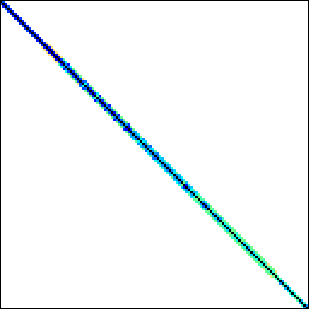
\includegraphics[width=\textwidth]{Cube_Coup_dt0}
        \caption{Cube\_Coup\_dt0}
    \end{subfigure}
    \hfill
    \begin{subfigure}[t]{0.45\textwidth}
        \centering
        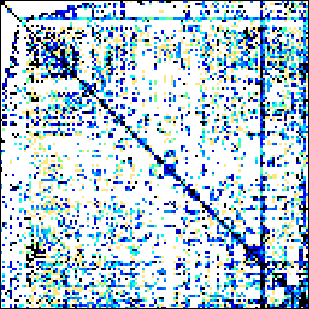
\includegraphics[width=\linewidth]{shermanACd}
        \caption{shermanACd}
    \end{subfigure}
    \caption{Well structured (a) and poorly structured (b) matrices.}
    \label{fig:Cube_Coup_dt0}
\end{figure}

\section{Shared Memory SpMV}
SpMV can be parallelized using the OpenMP directive \texttt{\#pragma omp parallel for}. By default, this tells OpenMP to use \texttt{static} scheduling when parallelizing the outer iteration loop. When static scheduling is used, the span of the iteration that each thread will execute is precomputed, and stays static, as the naming suggests. There are other scheduling options, such as \texttt{dynamic} and \texttt{guided}, which will be discussed in later sections.
\medskip

An implementation of shared memory SpMV is outlined below.
\medskip

\begin{algorithm}[H]
    \caption{Shared Memory CSR-based SpMV}
    \SetAlgoVlined
    \SetKwInOut{Input}{Input}
    \SetKwInOut{Output}{Output}
    \Input{\(A_{p},A_{j},A_{x},x\)}
    \Output{\(y\)\newline}

    \#pragma omp parallel for\\
    \For{\(i \gets 0\) \KwTo \(n\)}{
        sum \(\gets 0\)\\
        \For{\(j \gets A_{p}[i]\) \KwTo \(A_{p}[i+1]\)}{
            sum \( = \text{sum} + A_{x}[j] \cdot x[A_{j}[j]]\)\\
        }
        \(y[i] \gets\) sum
    }
    \label{alg:sharedmemoryspmv}
\end{algorithm}

\subsection{Scheduling options}
As seen in \autoref{alg:sharedmemoryspmv}, the outer loop is parallelized, which translates to dividing the rows of the matrix evenly among the threads. This work fine for well structured matrices, but for matrices with dense rows, such as the matrix shown in Figure \ref{fig:staticscheduling}, we obtain large imbalances in the computational load for each thread, which impacts performance. 

\begin{figure}[H]
    \centering
    \incfig{staticscheduling}
    \caption{staticscheduling}
    \label{fig:staticscheduling}
\end{figure}

\subsection{Dynamic scheduling}
With dynamic scheduling, OpenMP still precomputes the span of iterations, however threads are not assigned a specific set of iterations to execute. If thread \(A\) is assigned a set of sparse rows, and thread \(B\) is assigned a set of dense rows, then with static scheduling, \(A\) will be idle and not perform any computation while \(B\) is busy with its dense rows. With dynamic scheduling, iterations will be dynamically assigned to threads that are idle, which can distribute the workload more evenly in cases where the computational load of each iteration can differ. 
\medskip

At first glance, it might seem that this will fix the problem static schecduling poses in regards to workload imbalance. This can be the case on single socketed machines with few physical cores such as on a personal laptop, but as the systems that are used in this thesis are dual-socketed, and have a large number of physical cores, it is crucial to consider the impact that \textit{first touch policy} has.

\subsection{First touch policy}
In short, first touch policy means that the first thread to access a memory page will be the one to allocate it to its local memory. This means that if thread \(A\) accesses a memory page, and then thread \(B\) accesses the same memory page, thread \(B\) will not have access to the data in its local memory, and will have to access it from the main memory. This can lead to performance degradation if the data is accessed frequently, as accessing data from main memory is significantly slower than accessing it from local memory. 


\subsection{Performance impact of first touch policy}
As seen in table \ref{tab:latencynumbers}, accesses to main are significantly slower than accesses to say the L1 cache, and on dual-socketed nodes, accesses to main memory on the opposite socket have to be sent through the interlink, which is once again signicantly slower than accessing main memory. From this it becomes evident that using dynamic (or guided) scheduling is not a solution to the performance issues that might arise from poorly structured matrices.









% This algorithm can be parallelized using shared memory parallelization using OpenMPs \texttt{\#pragma omp parallel for} directive in the following manner:
% \medskip

% \begin{algorithm}[H]
%     \caption{Sequential CSR-based SpMV}
%     \SetAlgoVlined
%     \SetKwInOut{Input}{Input}
%     \SetKwInOut{Output}{Output}
%     \Input{\(A_{p},A_{j},A_{x},x\)}
%     \Output{\(y\)\newline}

%     \textbf{\#pragma omp parallel for}\\
%     \For{\(i \gets 0\) \KwTo \(n\)}{
%         \(y[i] \gets 0\)\\
%         \For{\(j \gets A_{p}[i]\) \KwTo \(A_{p}[i+1]\)}{
%             \(y[i] \gets y[i] + A_{x}[j] \cdot x[A_{j}[j]]\)\\
%         }
%     }
% \end{algorithm}

% \section{Computational Intensity}

\section{Distributed Memory SpMV}
This thesis examines the performance of SpMV in a hybrid environment combining distributed and shared memory. The matrix is divided among multiple nodes in a cluster, where each node has its own local memory. Within each node, OpenMP is used to parallelize the local SpMV computation. After completing local operations, nodes exchange data through the Message Passing Interface (MPI) to assemble the final result. 

\section{Load Balancing}
In a distributed memory system, it is important to partition the matrix so that the computational workload is evenly divided among the processes. This is typically achieved through the use of graph partitioning tools. A widely used tool for this purpose is METIS, which provides the function \texttt{METIS\_PartGraphKway}. Given a parameter \(nprocs\), representing the number of processes the program will run on, \texttt{METIS\_PartGraphKway} attempts to partition the graph into \(nprocs\) equally sized parts. Since finding an optimal partition is an NP-hard problem, METIS does not guarantee an optimal solution, but it produces high-quality approximations that are sufficient for practical use.

\subsection{Separator}
When a graph is partitioned into different parts, there will inevitably be some edges which strides across different partitions. The endpoints of these edges are called separators, and will become important when it comes to reducing the communication load of the SpMV computation.



\section{Distributed Memory CSR}










